%#!platex ./report.tex

 \section{Ka$B%A%c%M%k$rMQ$$$?>l9g$N7k2L(B}
   $B?^(B\ref{Ka_Result1}, $B?^(B\ref{Ka_Result2}$B$K(BKa$B%A%c%M%k$rF3F~$7$?:]$N7k2L$r<($9(B. $B?^Cf$N(BGausian$B$O%3%s%@%/%?%s%9J,I[MM<0$K(B
   $B%,%&%9J,I[$rMQ$$$F$*$j(B, Liner$B$O@~7AJ,I[$rMQ$$$?>l9g$N7k2L$G$"$k(B.
   $B$^$?(B-reduced$B$O$=$l$>$l$N%3%s%@%/%?%s%9J,I[MM<0$G(B, $B8DBNI>2A$K%3%s%@%/%?%s%9NL$X$N9MN8$rF3F~$7$?>l9g$N7k2L$G$"$k(B. \\
   $B%0%i%U>eIt$N5-9f$O3F(B${\Delta}t$$B$K$*$$$F(B, $B%&%'%k%A$N(Bt$B8!Dj(B($\alpha = 0.05$)$B$r9T$$M-0U:9$,$_$i$l$?$3$H$r(B
   $B<($7$F$$$k(B. $B5-9f(B($\star$)$B$OK\8&5f<jK!$N(BPassive$B$N7k2L$H(BGausian, Liner$B$N7k2L$rHf3S$7(B, $B$=$l$>$l$N?'$G<($7$F$$$k(B.
   $B5-9f(B($\#$)$B$O(BGausian$B$H(Breduced-Gausian, Liner$B$H(Breduced-Liner$B$NAH$G8!Dj$r9T$C$?7k2L$G$"$k(B.
   $B$^$?5-9f(B($+$)$B$O(Breduced-Gausian$B$H(Breduced-Liner$B$NAH$G8!Dj$r9T$C$?7k2L$r<($7$F$$$k(B. 
   \vspace{-0.5cm}
     \begin{figure}[H]
       \begin{subfigure}{0.5\columnwidth}
         \centering
         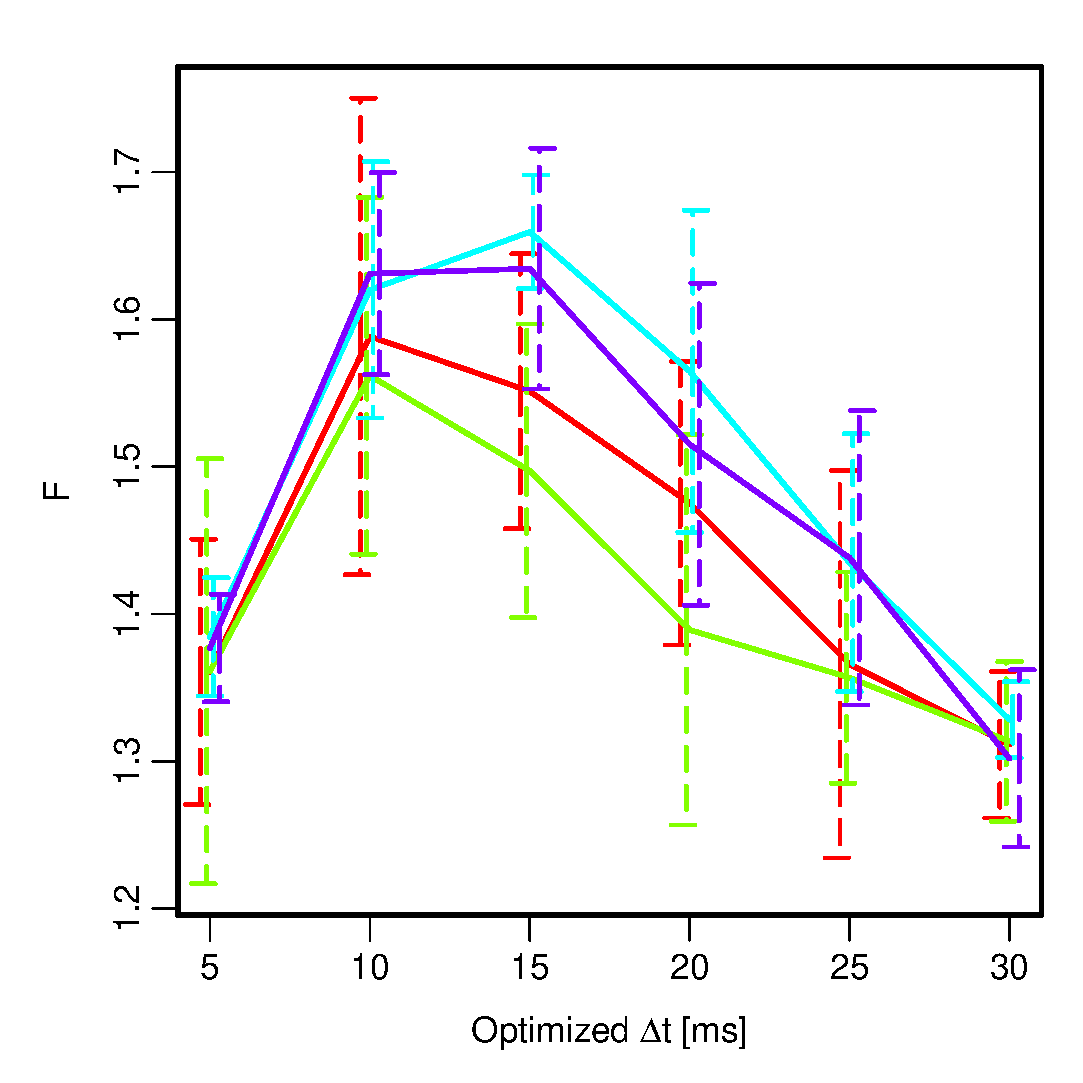
\includegraphics[width=0.8\columnwidth]{./Images_Result/k_test_F.eps}
         \caption{F}
         \label{k_F}
       \end{subfigure}
       \begin{subfigure}{0.5\columnwidth}
         \centering
         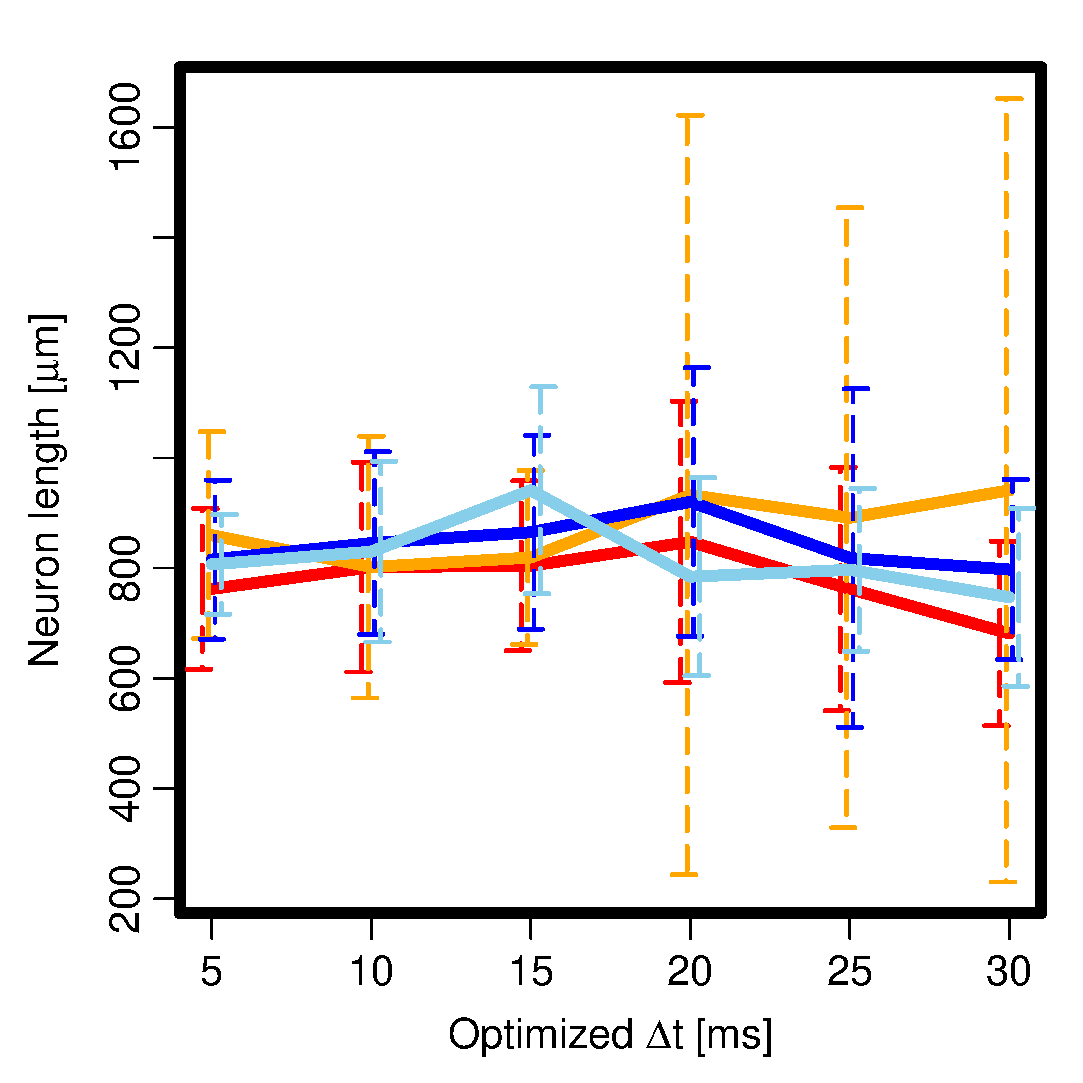
\includegraphics[width=0.8\columnwidth]{./Images_Result/k_test_TREE_length.eps} 
         \caption{$BD9$5(B}
         \label{k_TREE_length}
       \end{subfigure}

       \begin{subfigure}{0.5\columnwidth}
         \centering
         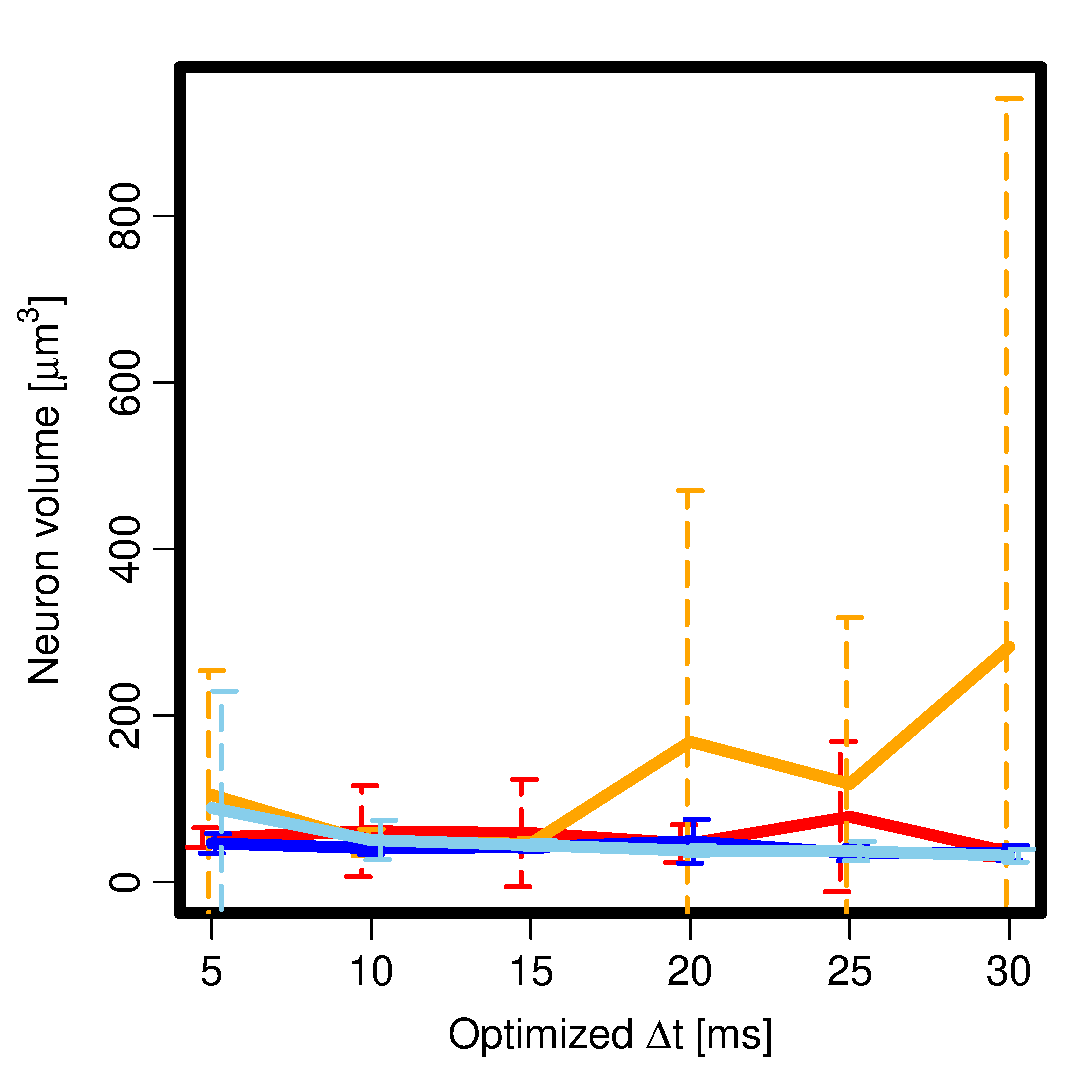
\includegraphics[width=0.8\columnwidth]{./Images_Result/k_test_TREE_volume.eps}
         \caption{$BBN@Q(B}
         \label{k_TREE_volume}
       \end{subfigure}
       \begin{subfigure}{0.5\columnwidth}
         \centering
         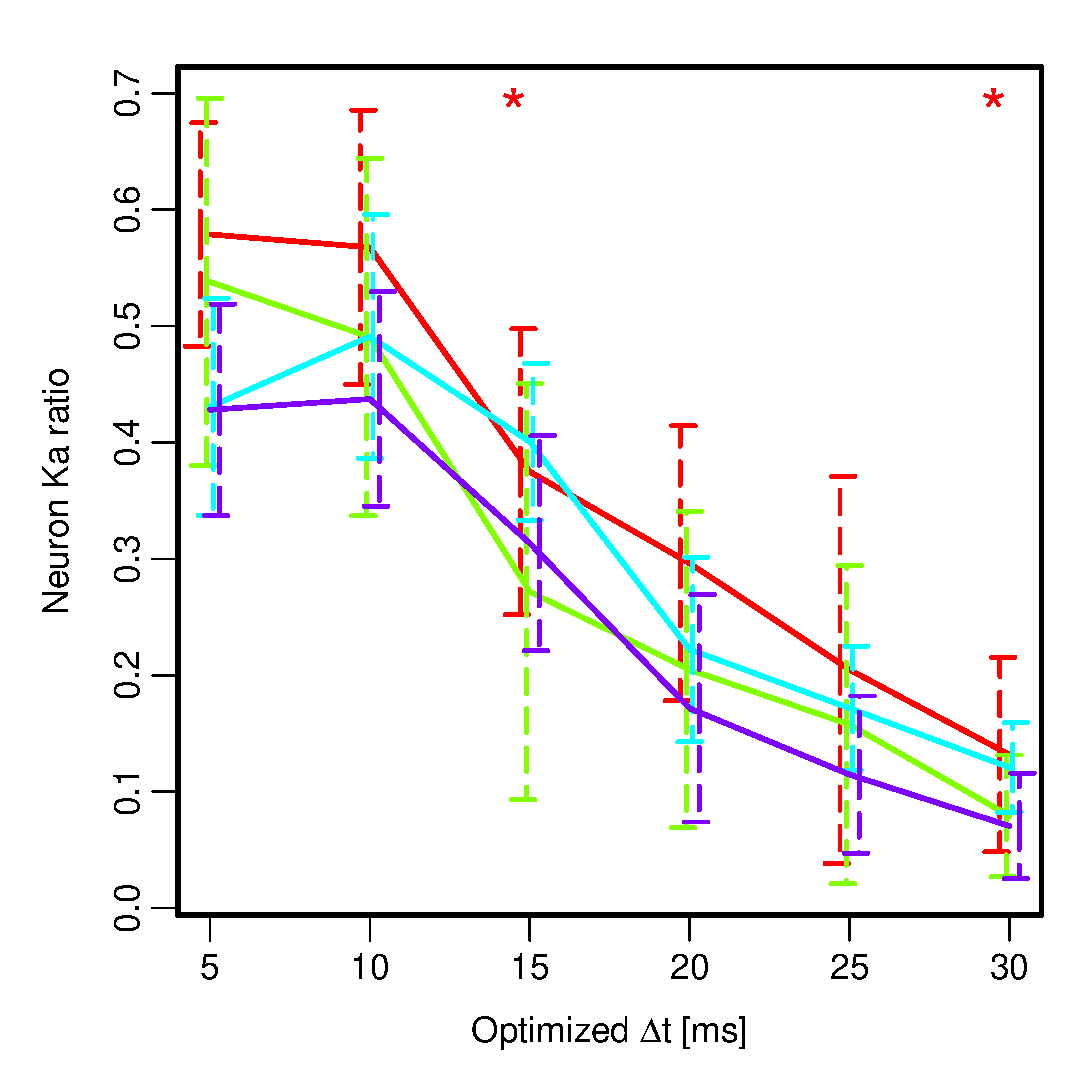
\includegraphics[width=0.8\columnwidth]{./Images_Result/k_test_TREE_K_ratio.eps}
         \caption{Ka$B%3%s%@%/%?%s%94^M-N((B}
         \label{k_TREE_K_ratio}
       \end{subfigure}

       \vspace{-0.3cm}
       \begin{subfigure}{0.5\columnwidth}
         \centering
         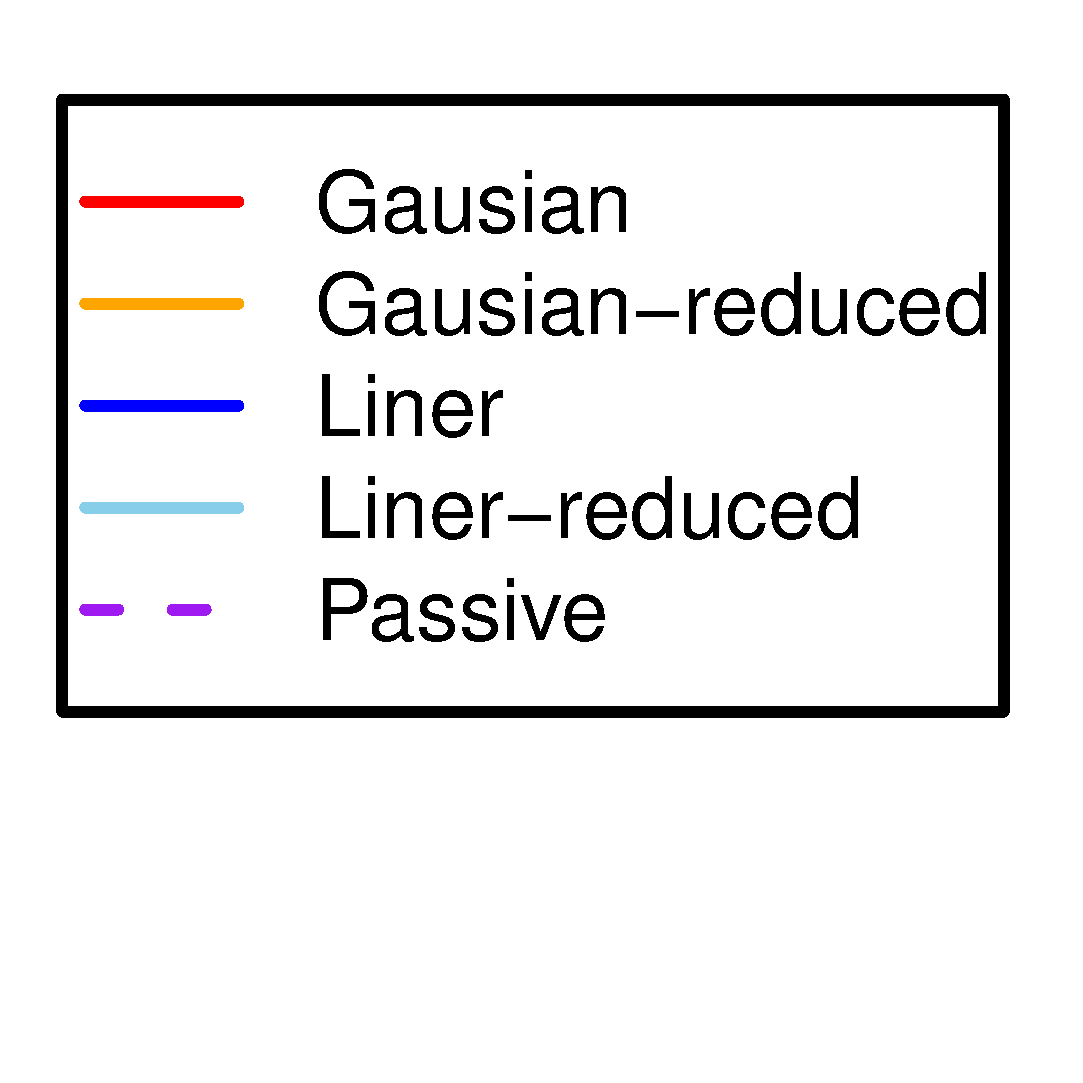
\includegraphics[width=0.6\columnwidth]{./Images_Result/k_test_legend.eps} 
       \end{subfigure}
       \begin{subfigure}{0.5\columnwidth}
         \centering
         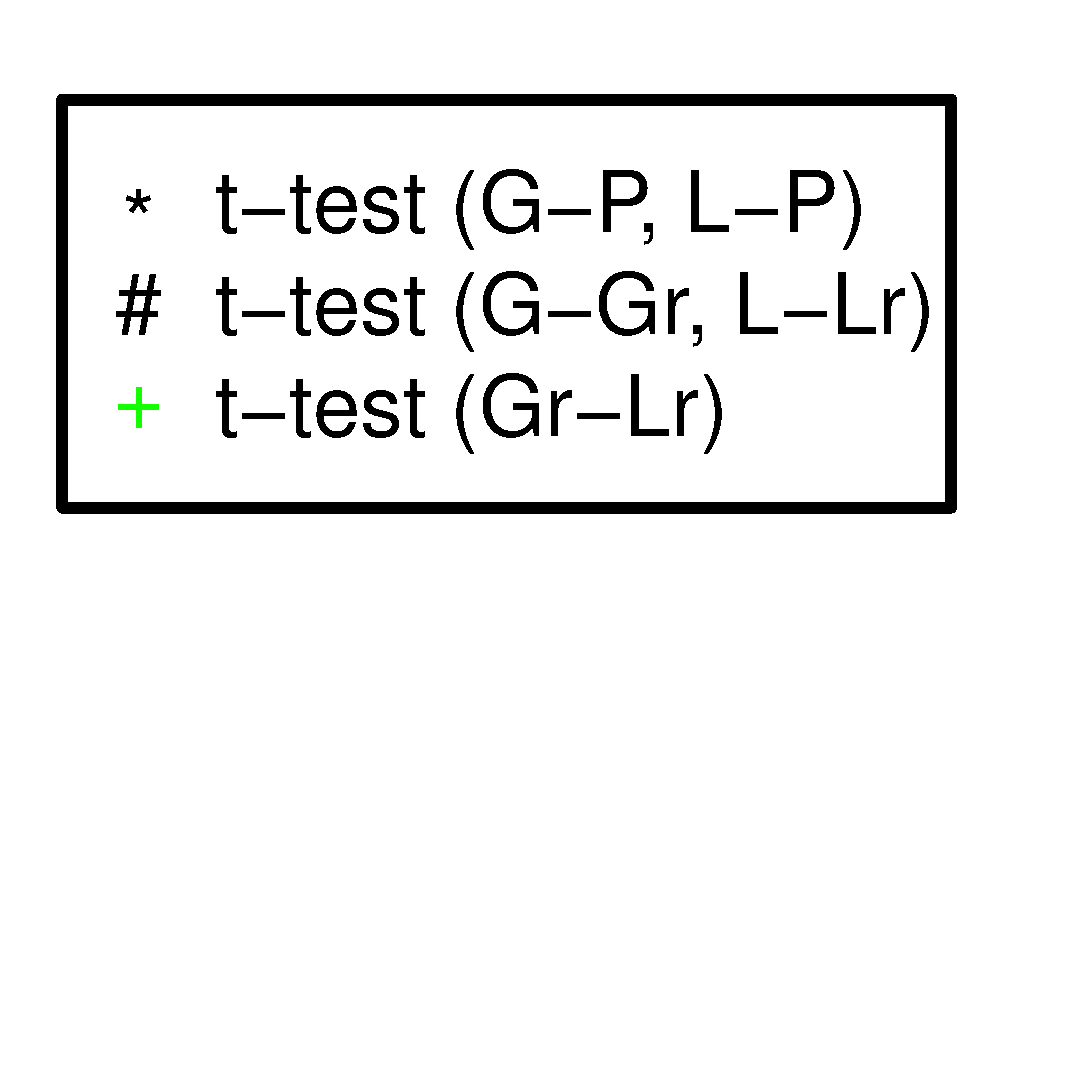
\includegraphics[width=0.6\columnwidth]{./Images_Result/test_legend.eps} 
       \end{subfigure}

       \vspace{-1.6cm}
       \caption{Ka$B%A%c%M%k$rF3F~$7$?:]$N7k2L(B1} %$B%Z!<%8%l%$%"%&%H$,7hDj$7$F$+$iHyD4@0$9$k(B
       \label{Ka_Result1}
     \end{figure}

     \begin{figure}[H]
       \begin{subfigure}{0.5\columnwidth}
         \centering
         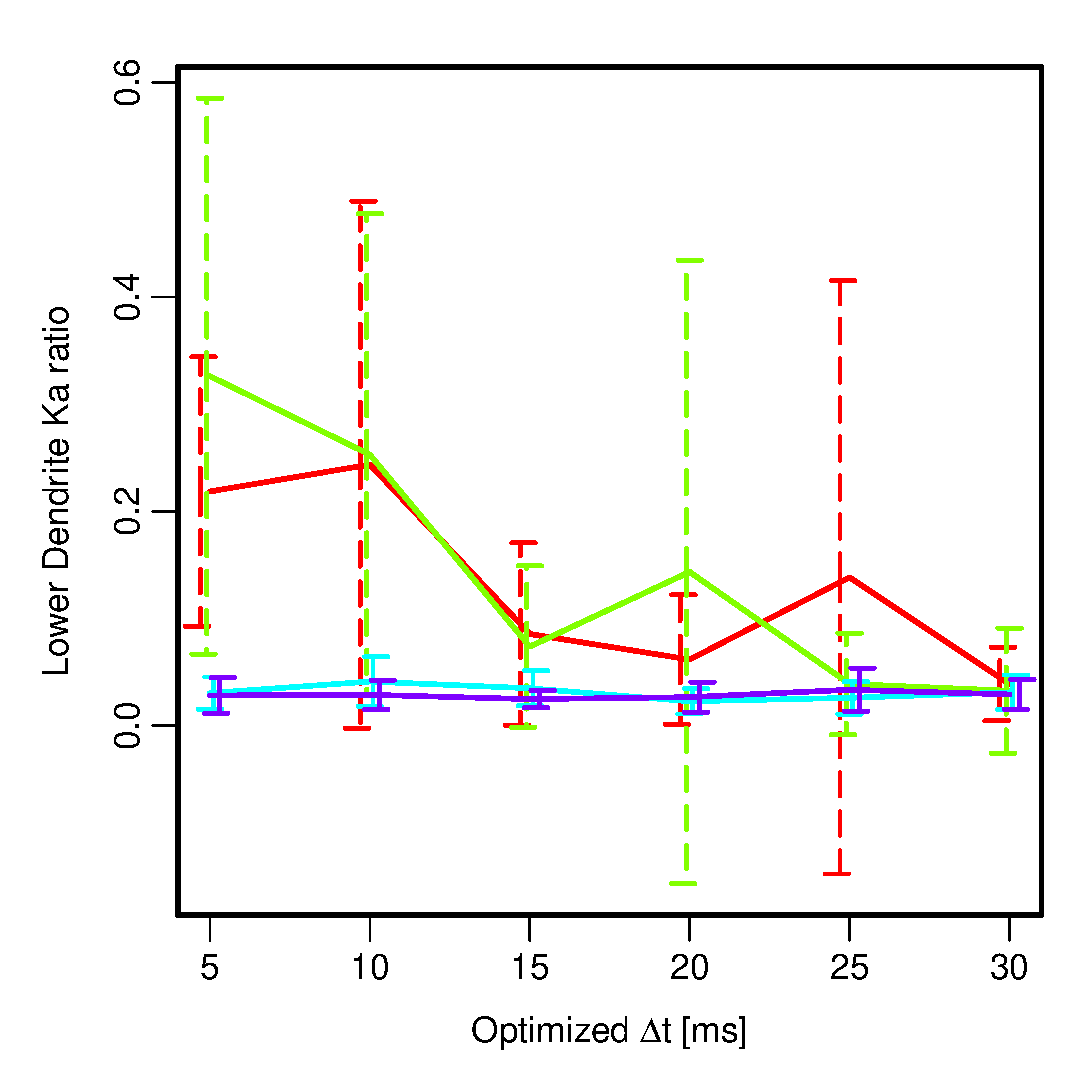
\includegraphics[width=0.8\columnwidth]{./Images_Result/k_test_Lower_K_ratio.eps}
         \caption{Lower Dendrite$B$N(BKa$B%3%s%@%/%?%s%94^M-N((B}
         \label{k_lower_k_ratio}
       \end{subfigure}
       \begin{subfigure}{0.5\columnwidth}
         \centering
         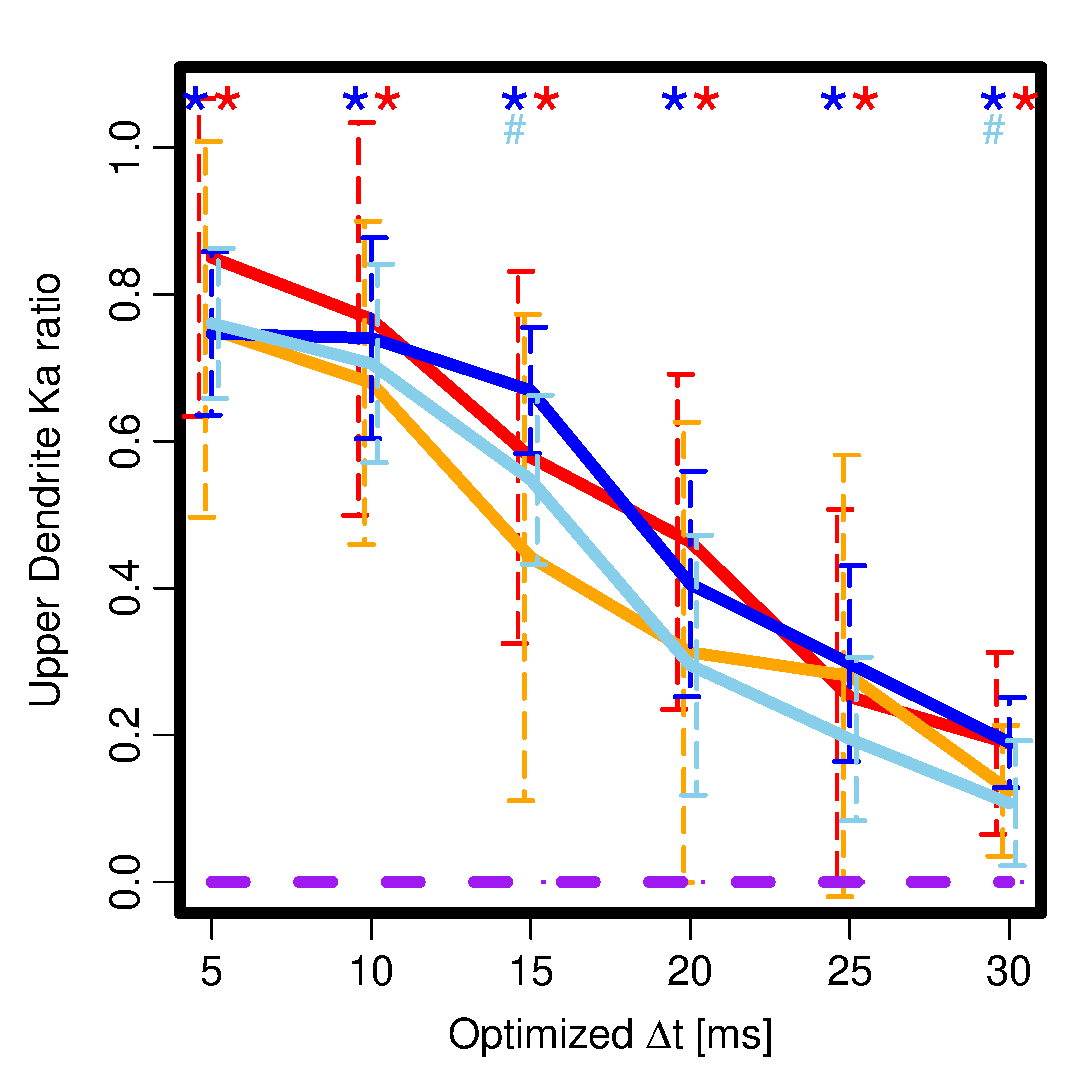
\includegraphics[width=0.8\columnwidth]{./Images_Result/k_test_Upper_K_ratio.eps}
         \caption{Upper Dendrite$B$N(BKa$B%3%s%@%/%?%s%94^M-N((B}
         \label{k_upper_k_ratio}
       \end{subfigure}

       \vspace{-0.3cm}
       \begin{subfigure}{0.5\columnwidth}
         \centering
         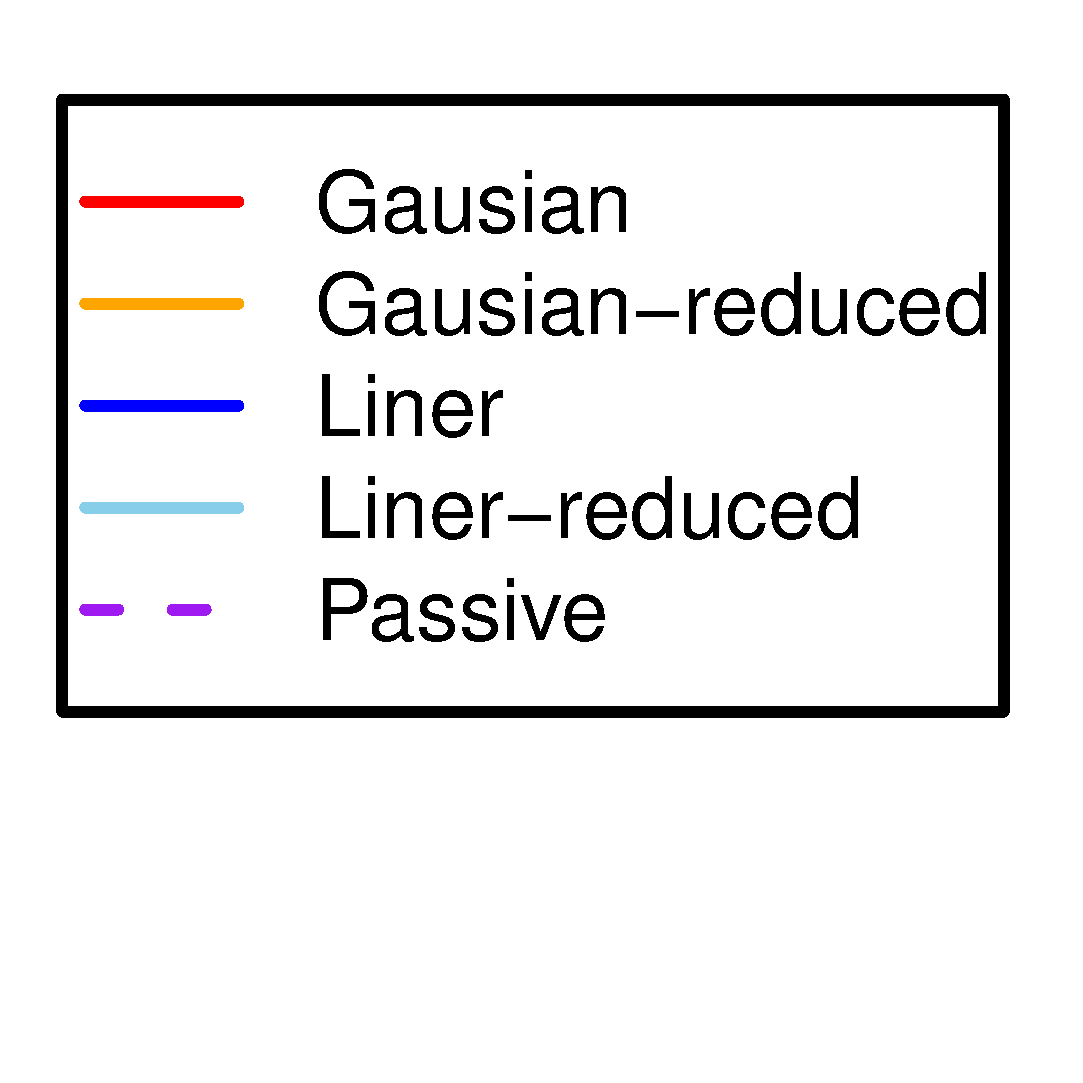
\includegraphics[width=0.6\columnwidth]{./Images_Result/k_test_legend.eps} 
       \end{subfigure}
       \begin{subfigure}{0.5\columnwidth}
         \centering
         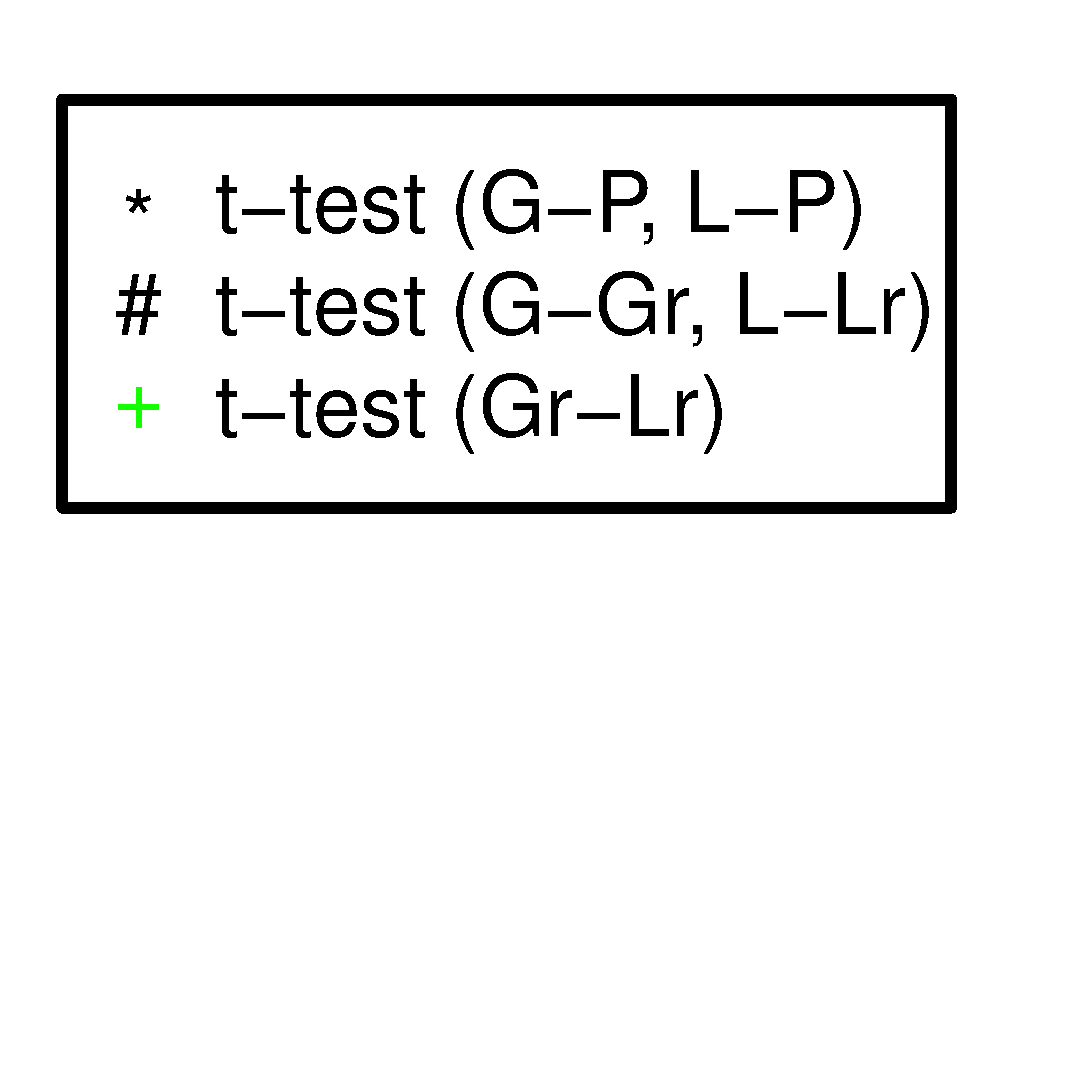
\includegraphics[width=0.6\columnwidth]{./Images_Result/test_legend.eps} 
       \end{subfigure}

       \vspace{-1.6cm}
       \caption{Ka$B%A%c%M%k$rF3F~$7$?:]$N7k2L(B2} %$B%Z!<%8%l%$%"%&%H$,7hDj$7$F$+$iHyD4@0$9$k(B
       \label{Ka_Result2}
     \end{figure}

  $B?^(B\ref{k_F}$B$h$j(BKa$B%3%s%@%/%?%s%9$rF3F~$7$?$3$H$G(BPassive$B$N>l9g$h$j$b(B$F$$BCM$,A}2C$7$F$$$k(B
  $B$3$H$,$o$+$k(B. $B@h9T8&5f$G$O(B${\Delta}t=5$[ms]$B$N$H$-$K:G$b9b$$(B$F$$BCM$,F@$i$l$F$$$?$,(B,
  $B$=$l$H$O0[$J$k7k2L$H$J$C$?(B. 
  $B?^(B\ref{k_TREE_K_ratio}$B$h$j%3%s%@%/%?%s%9$r9MN8$9$k>l9g$G$b?@7P:YK&(B
  $B$N(BKa$B%3%s%@%/%?%s%94^M-N($O$"$^$jJQ2=$,$J$$$3$H$,$o$+$k(B. \\

  %
  % $B$d$C$Q$j%3%s%@%/%?%s%9$rIT3h@-2=$7$?>l9g$H$N:90[$r=P$;$?J}$,$$$$(B
  %

  $B?^(B\ref{Ka_V}$B$O(BKa$B%3%s%@%/%?%s%9$rF3F~$7$?:]$N%7%_%e%l!<%7%g%s$N0lNc$G$"$k(B. 
  \begin{figure}[H]
    \centering
    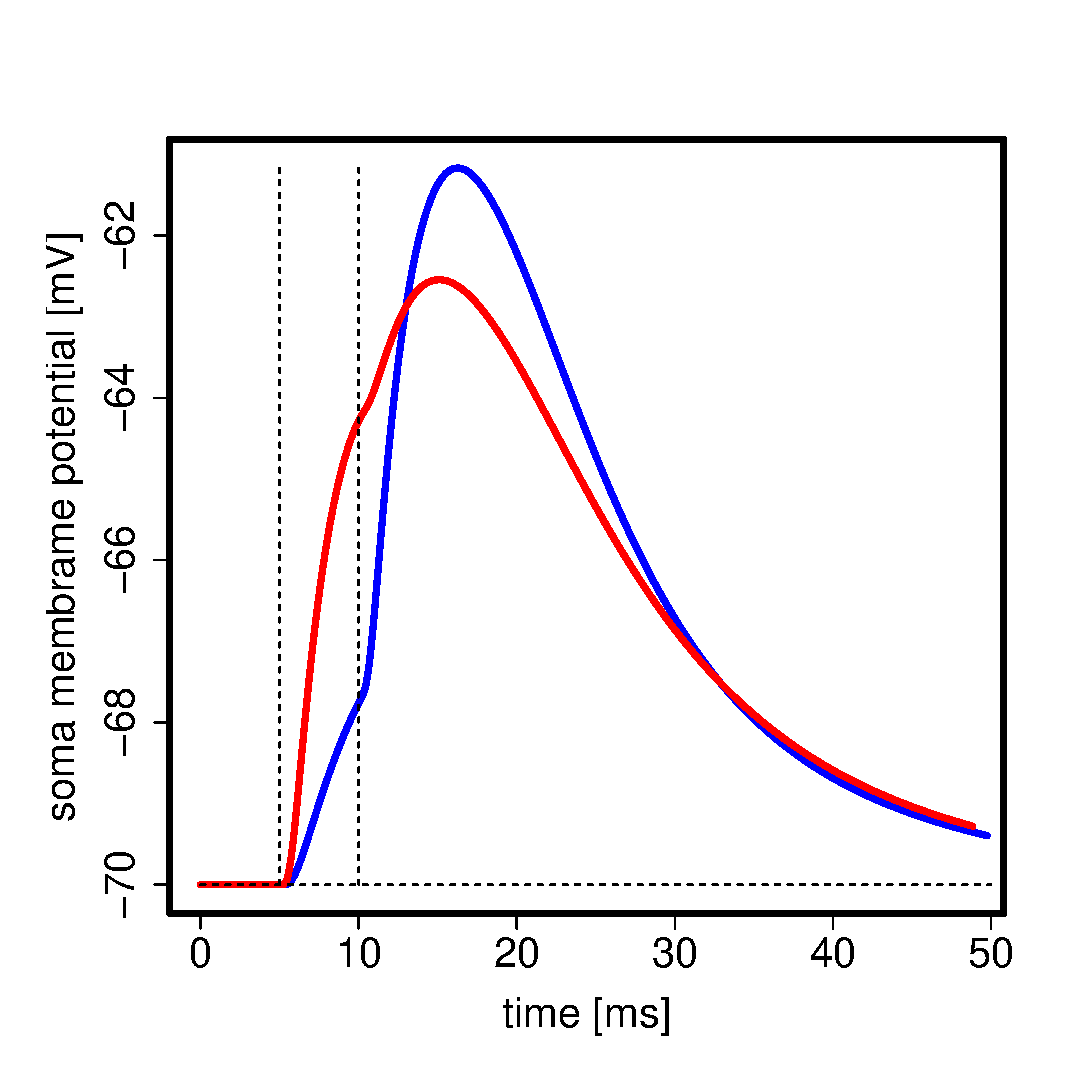
\includegraphics[width=0.4\columnwidth]{./Images_Result/k_gaus_somaV_dt5_C0.eps}
    \caption{Ka $B%7%_%e%l!<%7%g%sNc(B(${\Delta} = 5$[ms])}
    \label{Ka_V}
  \end{figure}
  %% $B?^(B\ref{k_morphos}$B$K:n@.$7$??@7P:YK&$N7ABVNc$r<($9(B. 
     
  %% \begin{figure}[H]
  %%   \begin{subfigure}{0.5\columnwidth}
  %%     \centering
  %%     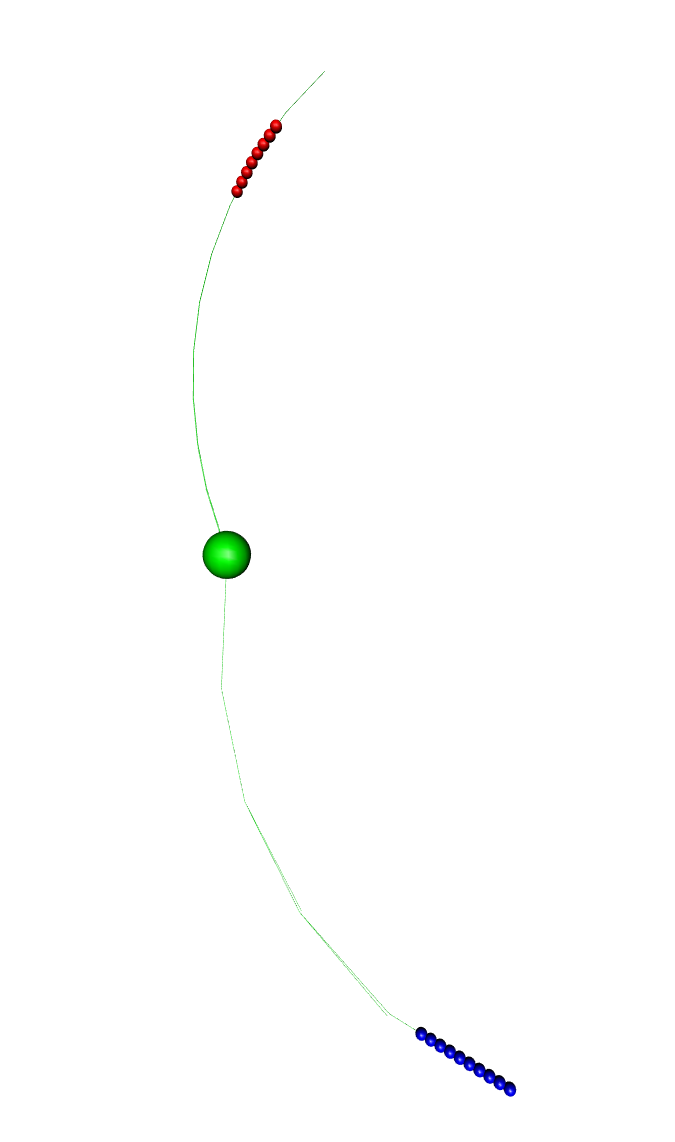
\includegraphics[width=0.5\columnwidth]{./Images_Result/k_liner_TREE_sample_dt5_C0.png} 
  %%     \caption{$B@~7AJ,I[(B}
  %%     \label{k_liner_morpho}
  %%   \end{subfigure}
  %%   \begin{subfigure}{0.5\columnwidth}
  %%     \centering
  %%     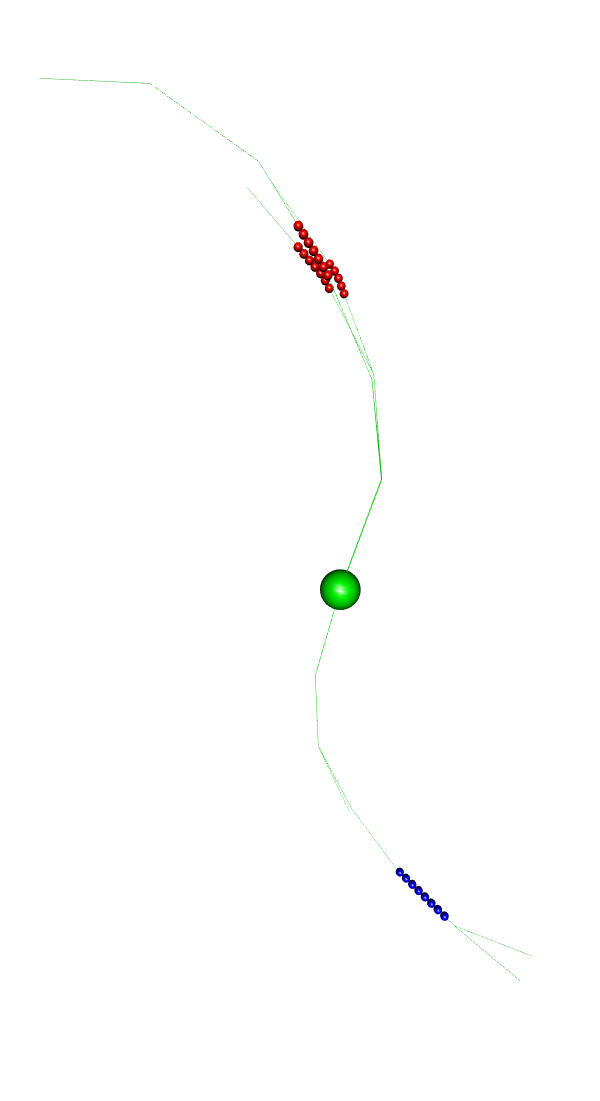
\includegraphics[width=0.5\columnwidth]{./Images_Result/k_gaus_TREE_sample_dt5_C0.png}
  %%     \caption{$B%,%&%9J,I[(B}
  %%     \label{k_gaus_morpho}
  %%   \end{subfigure}
  %%   \caption{Ka$B%3%s%@%/%?%s%9$rF3F~$7$??@7P:YK&$N7ABVNc(B}
  %%   \label{k_morphos}
  %% \end{figure}

   $B$^$?(B, $B?^(B\ref{k_Ka_dist}$B$K(B${\Delta}t = 5$[ms]$B$H$7$F:n@.$7$??@7P:YK&$N(B
   $B%3%s%@%/%?%s%9J,I[$r<($9(B.
   $B?^(B\ref{k_liner_dist}$B$O@~7AJ,I[$rMQ$$(B, $B?^(B\ref{k_gaus_dist}
   $B$O%,%&%9J,I[$rMQ$$$F$$$k(B. $B$^$??^(B\ref{k_liner_reduced_dist}$B$H(B
   $B?^(B\ref{k_gaus_reduced_dist}$B$O$=$l$>$l$N%3%s%@%/%?%s%9J,I[MM<0$G(B,
   $BI>2A<0$K$*$$$F%3%s%@%/%?%s%9$N9MN8$r9T$C$?>l9g$N7k2L$G$"$k(B. 

      \begin{figure}[H]
     \hspace*{-2cm}
     \begin{subfigure}{0.62\columnwidth}
       \centering
       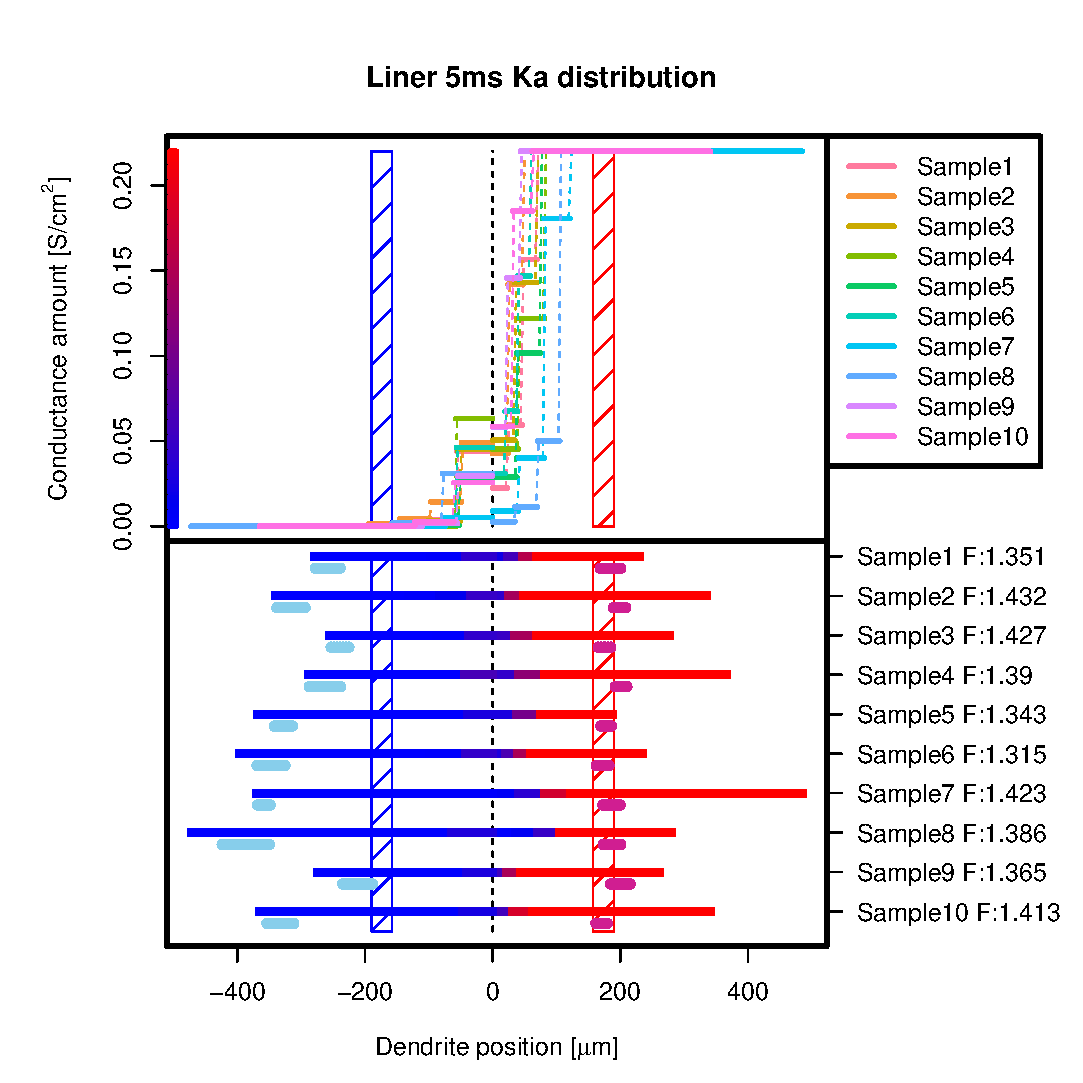
\includegraphics[width=\columnwidth]{./Images_Result/k_Rerative_liner_75_0_K_distribution_dt5.eps}
       \caption{$B@~7AJ,I[(B}
       \label{k_liner_dist}
     \end{subfigure}
     \begin{subfigure}{0.62\columnwidth}
       \centering
       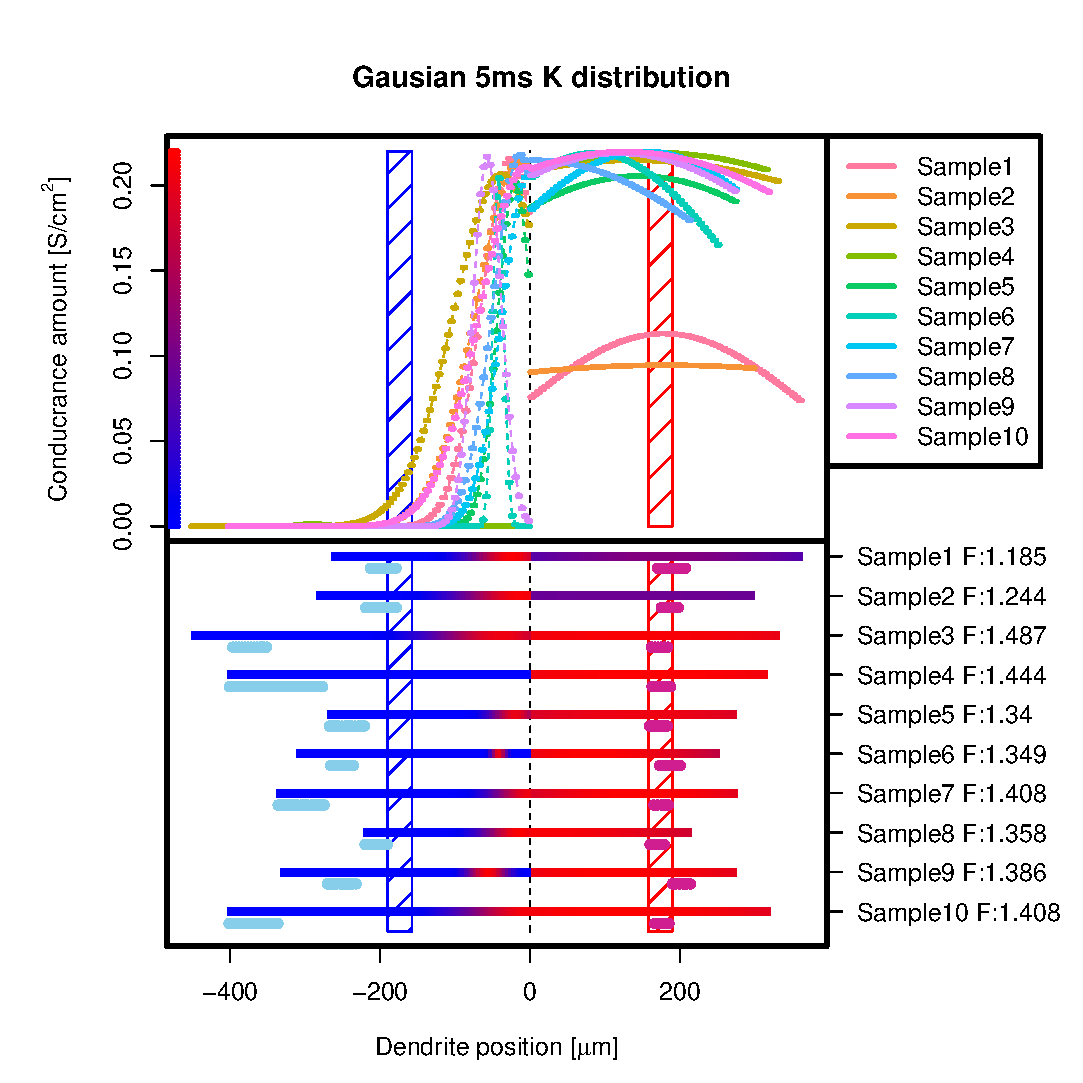
\includegraphics[width=\columnwidth]{./Images_Result/k_Rerative_Gaus_75_0_K_distribution_dt5.eps}
       \caption{$B%,%&%9J,I[(B}
       \label{k_gaus_dist}
     \end{subfigure}

     \hspace*{-2cm}
     \begin{subfigure}{0.62\columnwidth}
       \centering
       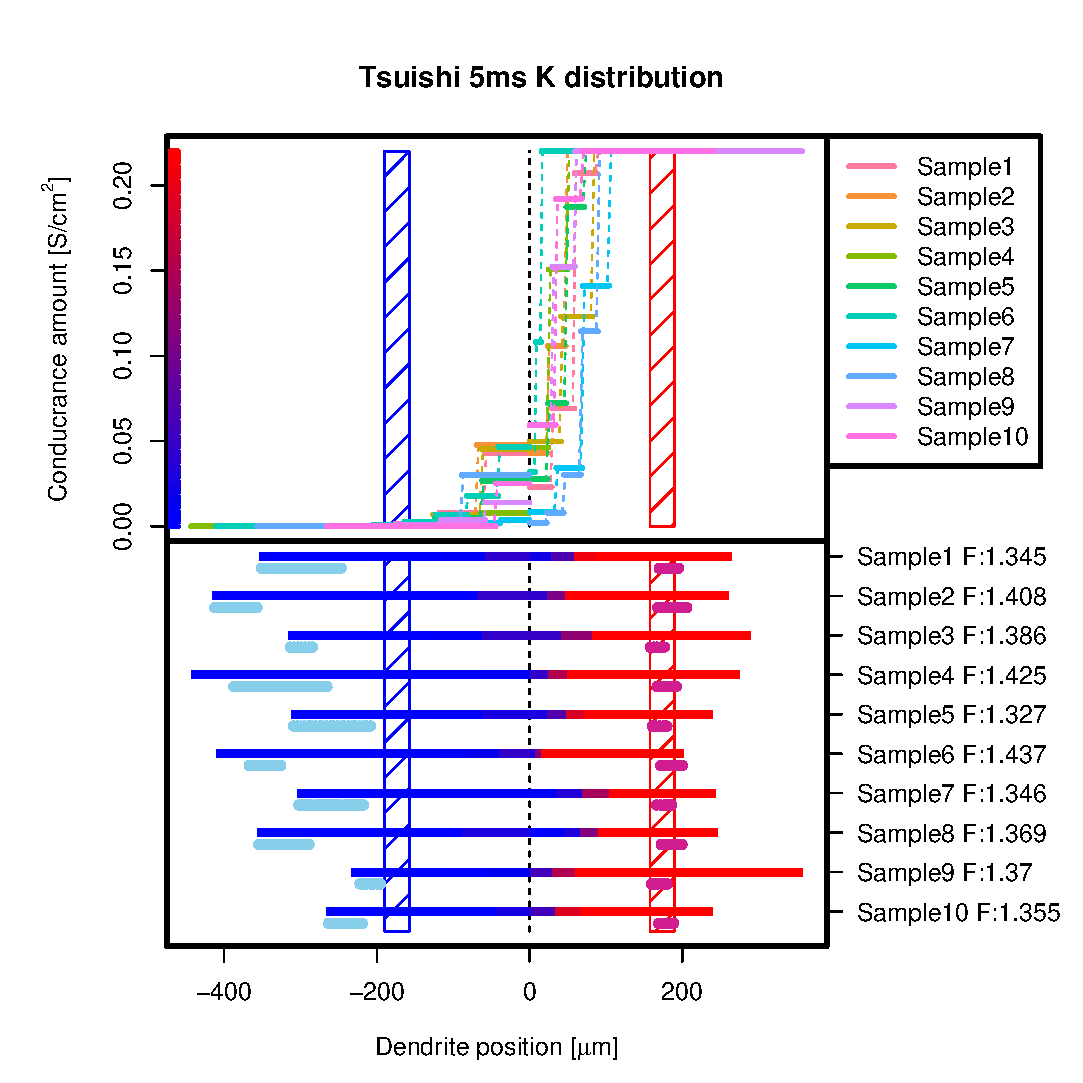
\includegraphics[width=\columnwidth]{./Images_Result/k_Rerative_liner_75_5_K_distribution_dt5.eps}
       \caption{$B@~7AJ,I[(B(reduced)}
       \label{k_liner_reduced_dist}
     \end{subfigure}
     \begin{subfigure}{0.62\columnwidth}
       \centering
       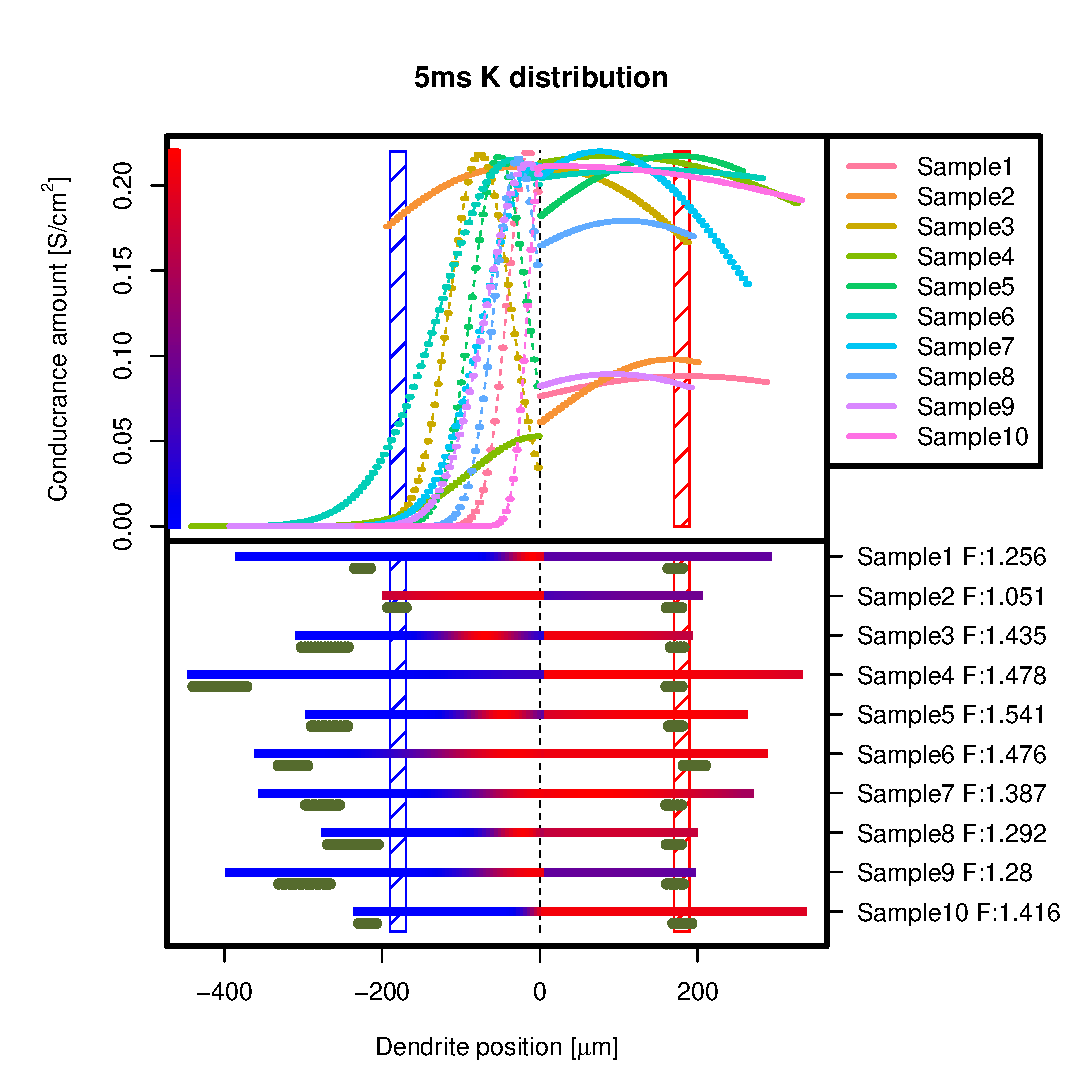
\includegraphics[width=\columnwidth]{./Images_Result/k_Rerative_Gaus_75_5_K_distribution_dt5.eps}
       \caption{$B%,%&%9J,I[(B(reduced)}
       \label{k_gaus_reduced_dist}
     \end{subfigure}
     
     \begin{subfigure}{\columnwidth}
       \centering
       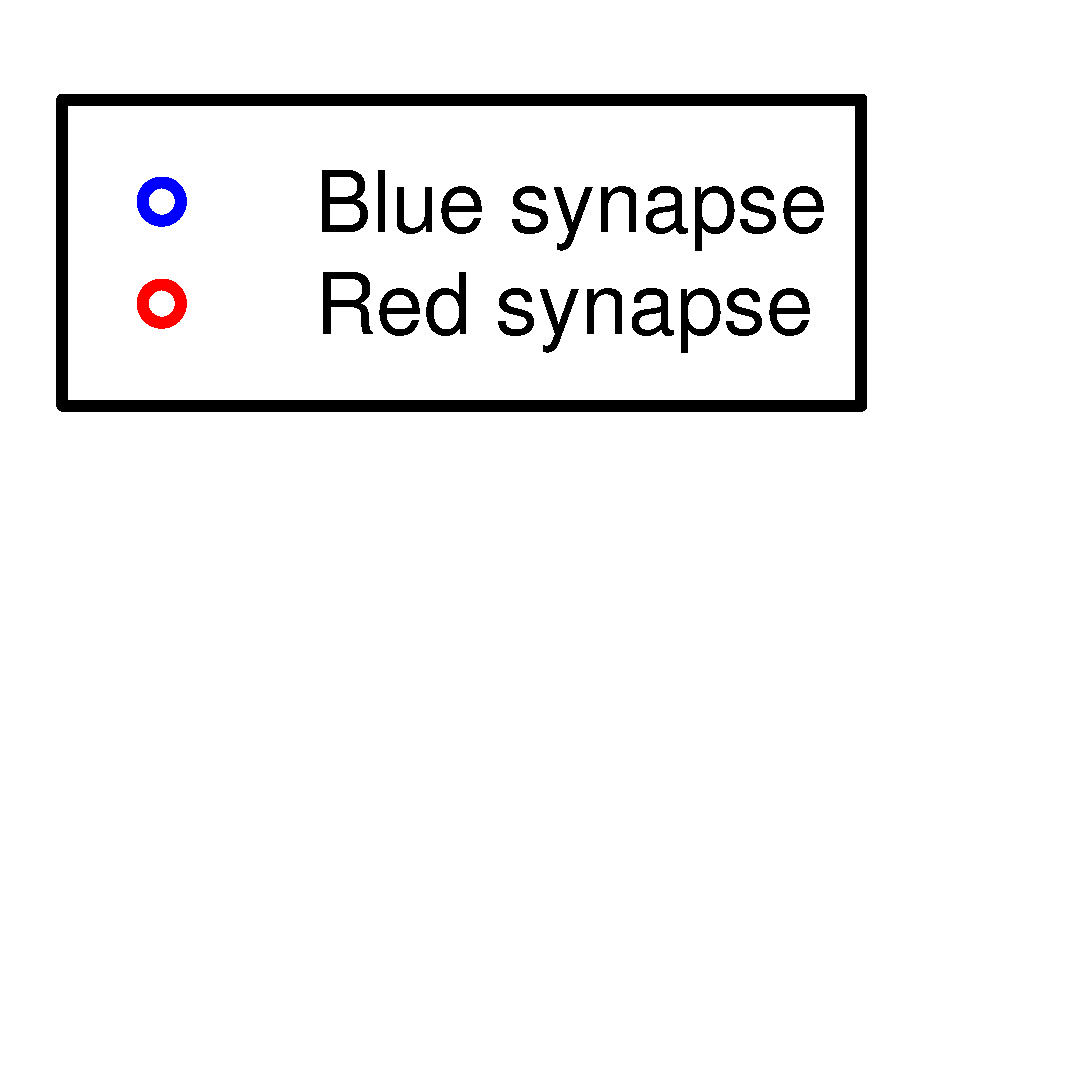
\includegraphics[width=0.35\columnwidth]{./Images_Result/Synapse_legend.eps} 
     \end{subfigure}
            
     \vspace{-3cm}
     \caption{${\Delta}t = 5$[ms], $B$G$N(BKa$B%3%s%@%/%?%s%9J,I[(B}
     \label{k_Ka_dist}
   \end{figure}

   $B?^(B\ref{k_gaus_reduced_dist}, $B?^(B\ref{k_upper_ratio}$B$+$i$o$+$k$h$&$K%,%&%9J,I[$rMQ$$$?>l9g(B
   $B$G$O(BUpper Dendrite$B$N:,85IU6a$G9b$$(BKa$B%3%s%@%/%?%s%9$NJ,I[$,8+$i$l$k(B.
   
